\documentclass{article}
\usepackage[utf8]{inputenc}
\usepackage[spanish]{babel}
\usepackage{listings}
\usepackage{graphicx}
\graphicspath{ {images/} }
\usepackage{cite}
\usepackage[backend=bibtex]{biblatex}
\addbibresource{references.bib}

\begin{document}

\begin{titlepage}
    \begin{center}
        \vspace*{1cm}
            
        \Huge
        \textbf{Taller memoria}
        
        \vspace{0.5cm}
        \LARGE
        Informatica 2
            
        \vspace{2.5cm}
            
        \textbf{ Mateo Restrepo Mesa }
        
        \newline
        
        \textbf{ C.C 1000919004}
            
        \vfill
            
        \vspace{0.8cm}
            
        \Large
        Despartamento de Ingeniería Electrónica y Telecomunicaciones\\
        Universidad de Antioquia\\
        Medellín\\
        Septiembre de 2020
            
    \end{center}
\end{titlepage}
\tableofcontents
\newpage

\section{Introducción}

Actualmente las computadoras se han vuelto muy importantes en la vida 
humana, es por ello que también se ha vuelto indispensable la realización o creación de 
herramientas que a su vez sean mejoradas en un futuro o ya hayan sido mejoradas, así mismo el día de hoy hablaremos sobre una de estas herramientas, 
la memoria es un dispositivo esencial en un computador ya que retiene o almacena información. 
También hablaremos sobre los tipos de memoria existentes, la diferencia de rapidez entre una memoria y otra y como se gestiona una memoria.
Por otro lado nos encontramos con una memoria virtual la cual se podría decir que es un tipo de memoria especial ya que se encarga de ejecutar los procesos que requieren más memoria de la que dispone el sistema, ya que en la memoria principal se mantendrá solo aquella memoria que el proceso esté utilizando y el resto en disco. De tal manera que las limitaciones de memoria física ya no existiría.

El objetivo de este trabajo es analizar con profundidad la memoria y sus diferentes funcionamientos, además conocer los tipos de memorias, sus características como la velocidad y capacidad. Con esta información expandiremos la comprensión de la memoria a una visión más amplia sobre la mejor utilización de este elemento en la computación, ayudando así a la programación y creación de algoritmos eficientes y útiles, logrando explotar al máximo el funcionamiento de la memoria.

Asi que en esté trabajo observaremos unas preguntas que nos hacemos acerca de la memoria, gracias a la  lectura  brindada por el profesor Augusto  Enrique  Salazar  Ramirez  Jimenez  en  su  texto \cite{funcionamiento} ”Como  funciona  la  memoria  de  un computador"
\newpage


\section{Desarrollo del taller} \label{contenido}

\subsection{Defina que es la memoria del computador.}
La memoria del computador es la parte fundamental en donde se procesa la información temporal tanto cómo la de los programas que se procesan o se van a procesar en un determinado momento, la memoria se trata del dispositivo donde se almacena temporalmente toda la información con la que trabajan los microprocesadores para procesarla y devolver los resultados que los usuarios requieren..

Se puede decir que la memoria es el cerebro del computador ya que esté es el que se encarga de transportar información y datos del disco duro al procesador, estos datos se ejecutan en el procesador y luego de que se termine o se cierre el proceso la memoria se encarga de devolver esa informacion al disco duro.

Asi es como funciona una memoria:
-Los programas y archivos se alojan en su unidad de almacenamiento.
-El procesador del sistema transfiere los datos de los programas desde la unidad de almacenamiento a la memoria para su acceso y uso a corto plazo.
-A continuación, el procesador accede a los datos desde la memoria, que es como el banco de espacio de trabajo disponible de su ordenador.

Para hablar de una manera mas tecnica, se puede citar a la pagina tutorialspoint para que nos defina como se compone una memoria, \cite{Memoria} "La memoria se divide en gran número de piezas pequeñas llamadas células. Cada ubicación o celda tiene una dirección única que varía desde cero hasta el tamaño de la memoria menos uno. Por ejemplo, si el ordenador tiene 64 k palabras, entonces esta unidad de memoria tiene 64 * 1024 = 65536 posiciones de memoria. La dirección de estos lugares varía de 0 a 65535"

\subsection{Mencione los tipos de memoria que conoce y haga una pequeña descripción de cada tipo.}
-Memoria RAM: La memoria RAM es la que se encarga de guardar y mantener abierto o en segundo plano los datos de una aplicación temporalmente,  tiene una capacidad limitada y los datos se eliminan cuando se apaga el suministro eléctrico y generalmente se compone de un semiconductor el cual es un elemento que tiene una conductividad eléctrica inferior a la de un conductor metálico pero superior a la de un buen aislante. \newline

\begin{figure}[h]
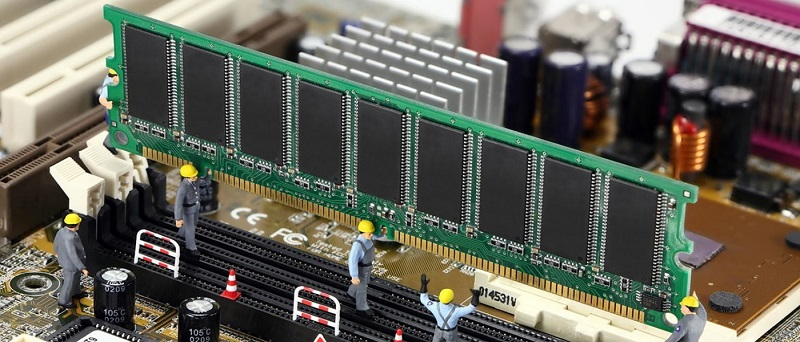
\includegraphics[width=6cm]{Memoria.jpg}
\centering
\caption{Memoria RAM}
\end{figure}

-Memoria ROM: Es la que se encarga de almacenar los datos de todas las aplicaciones y el sistema operativo, hablaremos de las dos unidades de ROM mas conocidos en la actualidad en un computador:

-Disco de estado mecanico (HDD) esta conformado por unos discos rígidos, recubiertos con material magnético. Sobre sus discos, se sitúa un cabezal de lectura/escritura que flota sobre una delgada lámina de aire generada por la rotación de los discso, debido a esto, está unidad de memoria ROM es lenta porqué para leer la información esté debe buscarlos en el lugar donde el cabezal escribio dicha información, por lo cual hace que esta unidad no sea del todo eficiente.

-Discos de estado solido (SSD), Estas unidades utilizan una memoria no volátil, para almacenar datos, en lugar de platos o discos magnéticos como lo es en los discos duros mecanicos, estos son mas resistentes y el tiempo de lectura de archivos es muy corto, esto debido a que un disco de estado solido no tiene partes moviles por lo cual poseen un menor tiempo de acceso a la información y menor tiempo de latencia.
\newline

\begin{figure}[h]
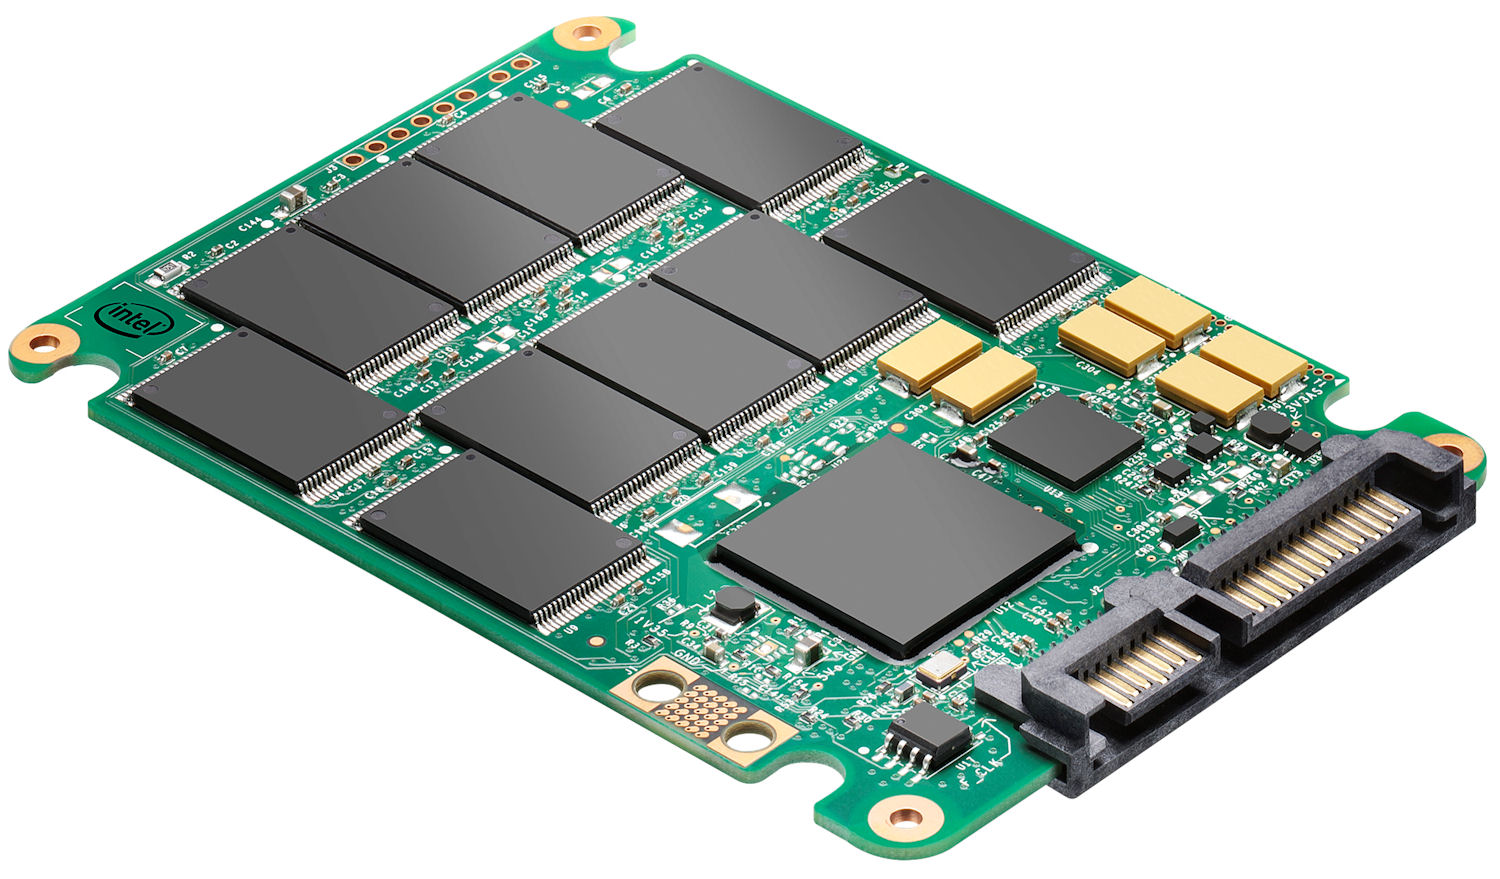
\includegraphics[width=4cm]{ssd.jpg}
\centering
\caption{Memoria ROM}
\end{figure} 

-Memoria cache: Área de almacenamiento dedicada a los datos usados o solicitados con más frecuencia para su recuperación a gran velocidad, está memoria sirve para almacenar temporalmente los datos recientemente procesados en una memoria auxiliar. esta memoria alterna se sitúa entre el CPU y la Memoria RAM, \cite{cache} "provee de un empuje adicional en tiempo y ahorro de recursos al sistema. De allí su nombre, que en inglés significa "escondite".
\newline

\begin{figure}[h]
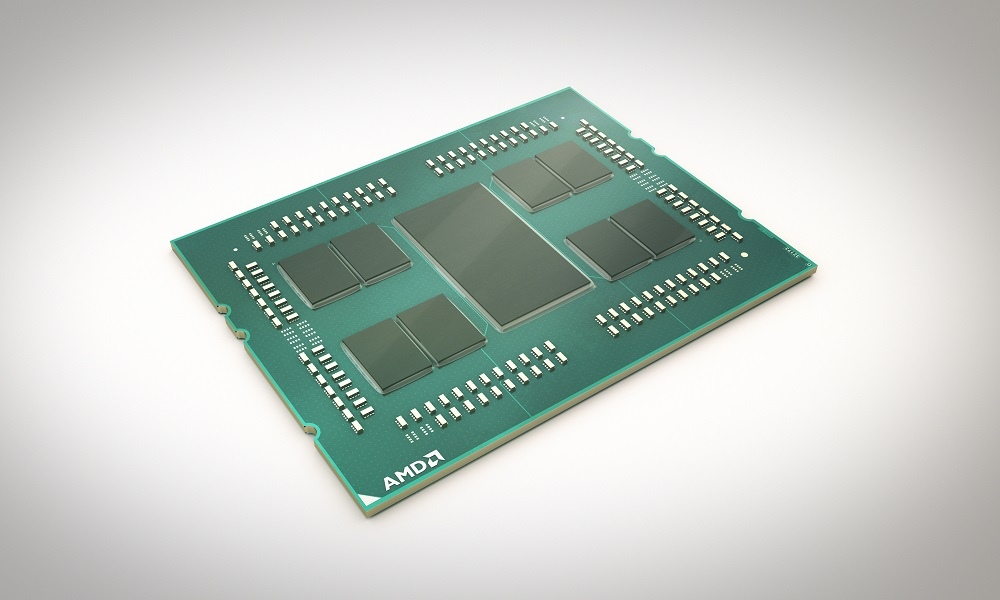
\includegraphics[width=4cm]{Cache.jpg}
\centering
\caption{Memoria cache}
\end{figure}
\newpage
-Memoria DRAM:Es un componente que permite el acceso a datos a corto plazo, puesto que las operaciones ejecutadas son de forma instantánea en el sistema, se basan casi siempre en acceso a datos a corto plazo.  \newline
\begin{figure}[h]
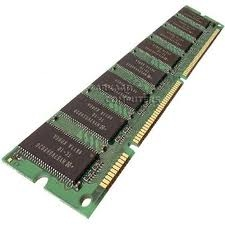
\includegraphics[width=4cm]{Dinamica.jpeg}
\centering
\caption{memoria DRAM}
\end{figure} 


-Memoria SRAM:Esta memoria está Basada en semiconductores, es capaz de mantener los datos, mientras esté alimentada, sin necesidad de un circuito de refresco. Sin embargo, sí son memorias volátiles, es decir que pierden la información si se les interrumpe la alimentación eléctrica. . \newline

\begin{figure}[h]
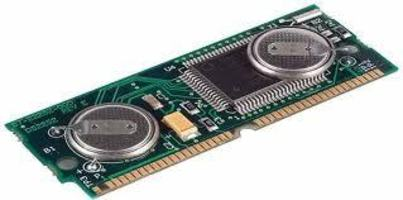
\includegraphics[width=4cm]{Estatica.jpg}
\centering
\caption{memoria SRAM}
\end{figure}

-Memoria Flash: Las memorias flash, permiten la lectura y escritura de datos, se pueden conectar en cualquier computador que tenga entrada (USB o SD) normalmente son portatiles debido a que son muy pequeñas y la ventaja es que tienen una gran capacidad pesé a su tamaño. \newline
\begin{figure}[h]
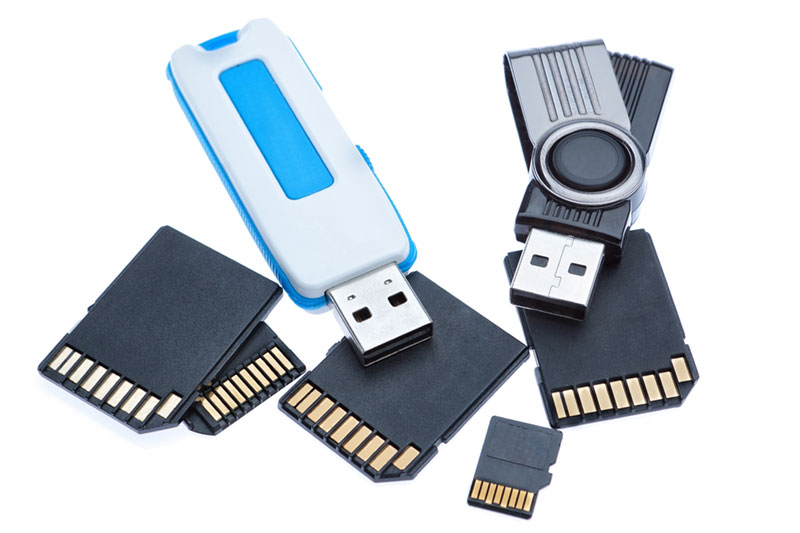
\includegraphics[width=4cm]{Flash.jpg}
\centering
\caption{memoria Flash}
\end{figure}

-Memoria Virtual: Es la memoria que se encarga de brindar tanto memoria para el usuario como para si misma, normalmente desde la unidad ROM, está memoria se ofrece normalmente cuando la memoria RAM llena su capacidad de almacenamiento. \newline
\begin{figure}[h]
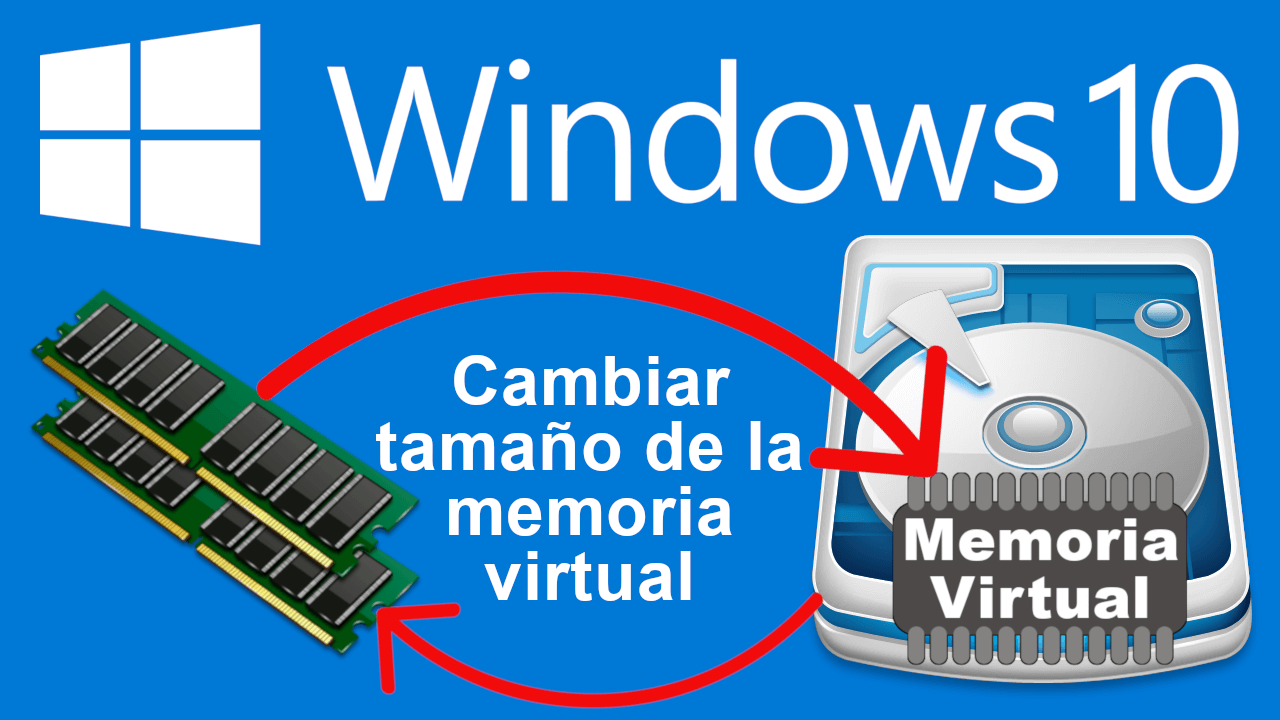
\includegraphics[width=6cm]{Virtual.png}
\centering
\caption{memoria Virtual}
\end{figure}

-Memoria VRAM: Es la memoria de video la cual permite ejecutar juegos o programas de alto nivel que requieran de muchos requisitos del sistema, en si es una memoria fundamental para un computador ya que es la que permite la alta calidad de imagen y refresco de está(FPS) los cuales son los fotogramas por segundo que son la cantidad de imágenes consecutivas que se muestran en pantalla por cada segundo. \newline
\begin{figure}[h]
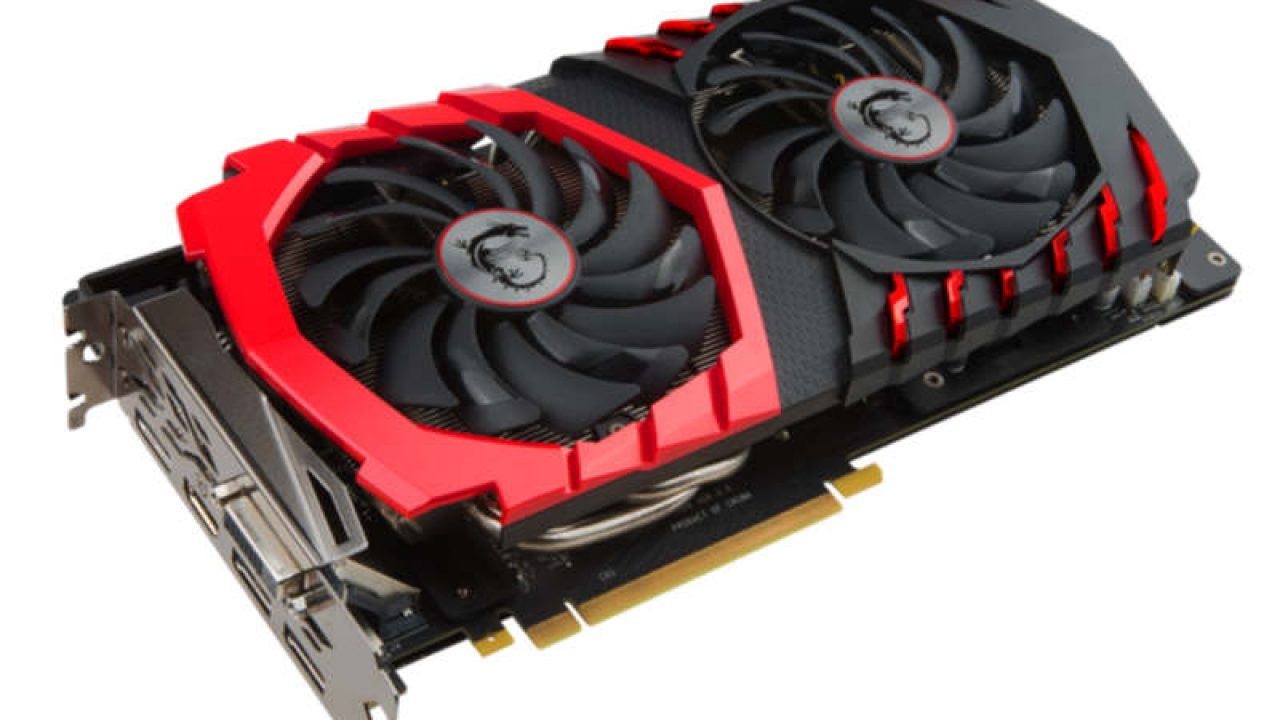
\includegraphics[width=6cm]{Vram.jpg}
\centering
\caption{memoria VRAM}
\end{figure}

\newpage
\subsection{Describa la manera como se gestiona la memoria en un computador.}

La gestión de la memoria principal de una computadora es una tarea de suma importancia para el funcionamiento de la misma.Existen varias formas de gestionar la memoria. Por lo común, la forma de gestión dependerá de la máquina virtual que se quiera proporcionar y del hardware subyacente, con independencia de la forma de gestión es necesario decidir qué estrategias se deben utilizar para obtener un rendimiento óptimo. Para poder gestionar la memoria adecuada y óptimamente el sistema operativo debe seguir las siguientes estrategias. \newline

1-Al iniciar el sistema operativo, los procesos de ejecucion del sistema se almacenan en el sistema. \newline
2-Todos los programas y procesos se gestionan en la memoria.\newline
3-Cuando la memoria llena su capacidad de frecuencia, empieza a liberar datos o aplicaciones para disminuir espacio. \newline
4-Se liberan secciones de memoria que ya no se utilizan para que estén disponibles para otros programas. \newline
5-Cuando se apaga el equipo, se borra toda la informacion de la memoria guardada.\newline


\subsection{¿Qué hace que una memoria sea más rápida que otra? ¿Por qué esto es importante?}

Esto depende de muchos factores. \newline

Lo que hace rápido una memoria de otra es la frecuencia de lectura de datos, la velocidad determina la rapidez a la que es capaz de trabajar la memoria RAM y afecta, junto con el bus de datos, a su ancho de banda. Una mayor velocidad permite realizar transferencias en menos tiempo. Las operaciones de almacenar, borrar y Re almacenar nueva información y datos se completarán más rápidamente, lo que en algunos casos puede marcar una diferencia importante de rendimiento. También es muy importante la capacidad de la memoria debido a que, si una aplicación pide una alta capacidad de almacenamiento para sus datos y tenemos una memoria con poca capacidad, esté programa se ejecutara de manera incorrecta, pero si tenemos una memoria de alta capacidad no tendremos problemas para ejecutar ese mismo programa.
\cite{mycomputer} "la memoria tiene una velocidad de reloj, y la CPU puede acceder más rápido a una memoria de velocidad más alta que a una memoria de velocidad más baja".

La pagina crucial.es, nos regala una recomendacion \cite{uso} "La velocidad y cantidad de memoria instalada ayuda a calcular la rapidez a la que funcionarán las aplicaciones, y a saber hasta qué punto su ordenador será eficaz realizando múltiples tareas. Actualizar la memoria de su sistema es una de las formas más fáciles y rentables de aumentar su rendimiento general", esta pagina nos dice que la cantidad de memoria instalada en nuestra computadora deprende de que tan eficaz se va a desempeñar está en diferentes tareas y que por eso es bueno poner atencion y preguntarnos ¿Para que usaré mi ordenador?, al tener claro esta pregunta la memoria influira un papel muy importante para el buen rendimiento del uso que le otorgaras al equipo.

\section{Conclusión} \label{conclulsion}

Así mismo, sabiendo que tipo memorias existen y para que se utilizan, podemos decir que la memoria es una de las partes fundamentales de un equipo electronico, cabe recalcar que sin una memoria ningún dispositivo encendería ya que la memoria se encarga de distribuir información de un lugar a otro y también se encarga de almacenarla, por decirlo de una manera abstracta, la memoria es el cerebro del computador, eso quiere decir que es la que facilita que un computador realice diferentes operaciones simultáneamente. \newline


\bibliographystyle{IEEEtran}
\printbibliography

\end{document}
